\section{number lines}

\begin{tikzpicture}
    \tkzInit[xmax=6,xstep=1]
    \tkzDrawX[left space=1, right space=1, text=blue, color=red, label=$t$,]
    \tkzLabelX[text=blue,below = 3pt]

    \myDot{2}{A}{solid}
    \myDot{4}{B}{empty}
\end{tikzpicture}

\noindent
\begin{tikzpicture}
    \tkzInit[xmax=6,xstep=1]
    \tkzDrawX[left space=1, right space=1, label={},]

    \myDot{2}{A}{empty}
    \myDot{4}{B}{solid}
    \tkzLabelPoint[below=2pt,black](A){$2$}
    \tkzLabelPoint[below=2pt,black](B){$4$}

    \tkzDefPoint(3,0){P-middle}
    \tkzLabelPoint[below=2pt,black](P-middle){{\tiny X}}
\end{tikzpicture}


\noindent
\begin{tikzpicture}
    \tkzInit[xmax=6,xstep=1]
    \tkzDrawX[left space=1, right space=1, label={}, ]

    \myBetweenSegment{2,0}{A}{empty}{4,0}{B}{solid}
\end{tikzpicture}



\noindent
\begin{tikzpicture}
    \tkzInit[xmax=6,xstep=1]
    \tkzDrawX[left space=1, right space=1, label={},]

    \myDotArrow{2}{A}{empty}{left}
    \myDotArrow{4}{A}{empty}{right}
\end{tikzpicture}



\noindent
\begin{tikzpicture}
    \tkzInit[xmax=6,xstep=1]
    \tkzDrawX[left space=1, right space=1, label={},]

    \myDotArrow{1}{A}{empty}{left}
    \myBetweenSegment{2,0}{B}{empty}{4.5,0}{C}{solid}
    \myDotArrow{6}{D}{solid}{right}
\end{tikzpicture}



\noindent
\begin{tikzpicture}
    \tkzInit[xmax=6,xstep=1]
    \tkzDrawX[left space=1, right space=1, label={},]

    \myDotArrow{4}[0.2]{A}{empty}{left}[4]
    \myDotArrow{2}[-0.2]{D}{solid}{right}[4]
\end{tikzpicture}
